\chapter{Die starke Wechselwirkung}
\begin{itemize}
\item[$\ra$]  bindet Nukleonen im Atomkern
\item[$\ra$] bindet Quarks in Hadronen
$\Ra$ Starke WW ist auf Quark/Gluon-Niveau theoretisch exakt beschreibbar
\end{itemize}
\section{Grundlegende Struktur}
Theorie der starken WW: Quantenchromodynamik\\
\glqq chromo\grqq{} wegen der Farbe (von Farbladungen)
\begin{figure}[!ht]
\centering
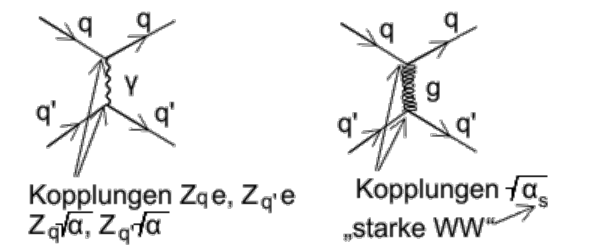
\includegraphics[width=.6\textwidth]{imgs/ep5-fig-7-1.pdf}
\caption{Feynmandiagramme zum Vergleich der starken und elm. WW \label{fig:7.1}}
\end{figure}
\begin{itemize}
\item[$\lt$] Gluonen sind masselos und koppeln an Farbladungen
\item[$\lt$] Es gibt 3 Farbladungen: r = rot, g = grün und b= blau
\item Theoretischer Hintergrund: Lokale Eichinvarianz\\
$\Ra$ fordere Invarianz unter:
\begin{align}
\text{elm. } & \Psi \ra \underbrace{e^{i\Phi\lb x_\mu\rb  } \Psi}_{\in Li(1)} & \Ra \ 1 \text{ \glqq Eichfeld\grqq{} = Photon}\\
\text{stark } & \Psi \begin{pmatrix}
r\\g\\b\end{pmatrix} \ra \underbrace{C\lb x_\mu\rb }_{\in SU(3)} \Psi \begin{pmatrix}r\\g\\b\end{pmatrix} & \Ra \ 8 \text{ Eichfelder = Gluonen, farbgeladen}
\end{align}
\item \tb{Farbladungen}
\begin{itemize}
\item[$\lt$] alle Leptonen, $\gamma$, $Z$, $W^{\pm}$ = 0
\item[$\lt$] alle Quarks: r,g,b
\item[$\lt$] alle Antiquarks: $\mr{\bar{r}, \bar{g}, \bar{b}}$
\item[$\lt$] alle Gluonen: $\mr{r\bar{g}, b \bar{r}, \dots}$
\newpage
\begin{figure}[!ht]
\centering
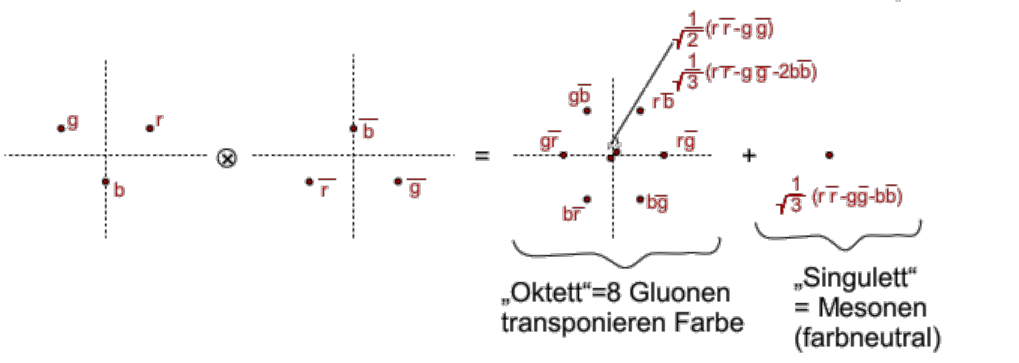
\includegraphics[width=.75\textwidth]{imgs/ep5-fig-7-2.pdf}
\caption{Kombination von Farbe und Antifarbe\label{fig:7.2}}
\end{figure}

\end{itemize}
\item Hadronen sind farbneutrale gebundene Systeme
\begin{itemize}
\item[$\lt$] Mesonen $\ket{q\bar{q}}$
\item[$\lt$] Baryonen $\ket{qqq}$
\item[$\lt$] \glqq Pentaquarks\grqq{} $\ket{qqqq\bar{q}}$
\item[$\lt$] \glqq Glueballs\grqq{} $\ket{gg}, \ \ket{ggg}$
\item Achtung Pentaquarks und Glueballs konnten noch nicht nachgewiesen werden!
\begin{figure}[!ht]
\centering
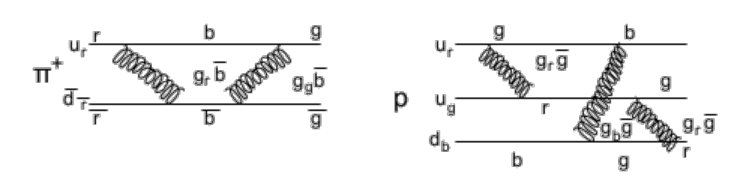
\includegraphics[width=.75\textwidth]{imgs/ep5-fig-7-3.pdf}
\caption{Skizze zur Farbladungserhaltung an jedem Vertex\label{fig:7.3}}
\end{figure}
\end{itemize}
\item Gluonen tragen Farbe

\begin{figure}[!ht]
\centering
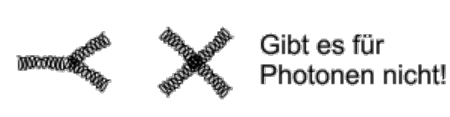
\includegraphics[width=.4\textwidth]{imgs/ep5-fig-7-4Gluonen.pdf}
\caption{Selbstwechselwirkung von Gluonen\label{fig:7.glue}}
\end{figure}

\item Farbgeladenen frei Teilchen (Quarks, Gluonen, Diquarks, \dots ) gibt es nicht\\
$\lt$ Confinement (\glqq Eingeschlossenheit\grqq)
\end{itemize}
\newpage
\section{Evidenzen für Gluonen und Farbe}
\begin{itemize}
\item \tb{Gluonen}
\begin{enumerate}
\item \tb{Tiefinelastische eN-Streuung}
\begin{align}
\int_0^1 \sum{q \text{ in } p } x q_i (x) \Pa x \approx 0.5
\end{align}
\begin{itemize}
\item[$\Ra$] Weitere \glqq Teilchensorte\grqq{} im Nukleon, mit der $e^-$ nicht wechselwirkt
\item[$\Ra$] elektrisch neutral
\end{itemize}
\item \tb{Jets}\\
\glqq Teilchenbündel\grqq\ in Richtung von Quarks oder Gluonen im Endzustand

\begin{minipage}[c]{.39\textwidth}
\captionsetup{type=figure}
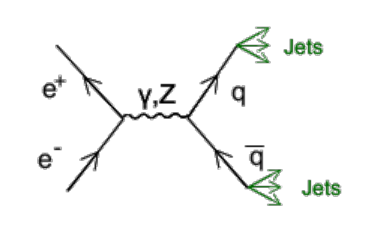
\includegraphics[width=\textwidth]{imgs/ep5-fig-7-4.pdf}
\captionof{figure}{Bsp.1: Feynmandiagramm für $e^+e^- \rightarrow q\bar{q}$ \label{fig:7.4}}
\end{minipage}
\begin{minipage}[c]{.39\textwidth}
\captionsetup{type=figure}
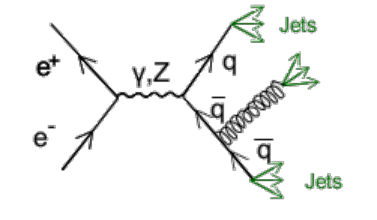
\includegraphics[width=\textwidth]{imgs/ep5-fig-7-5.pdf}
\captionof{figure}{Bsp.2: Feynmandiagramm für $e^+e^- \rightarrow q\bar{q}g$ \label{fig:7.5}}
\end{minipage}

\begin{itemize}
\item[$\rightarrow$] Entstehung von Jets oder auch von Baryonen
\item[$\rightarrow$] nur möglich, wenn einer der Jets von einem Gluon stammt
\item[$\rightarrow$] entdeckt 1979 am DESY
\end{itemize}

\begin{minipage}[c]{.39\textwidth}
\captionsetup{type=figure}
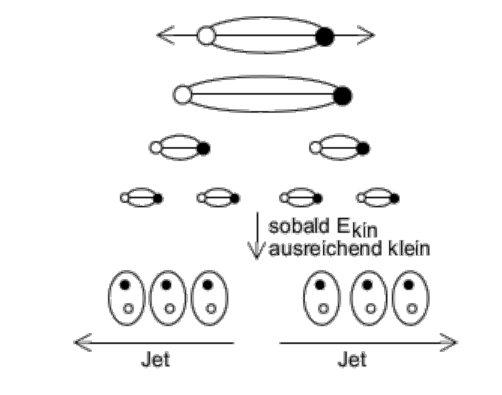
\includegraphics[width=\textwidth]{imgs/ep5-fig-7-6.pdf}
\captionof{figure}{Jet-Entstehung: für $e^+e^-$ entstehen 3 Jets \label{fig:7.6}}
\end{minipage}
\begin{minipage}[c]{.39\textwidth}
\captionsetup{type=figure}
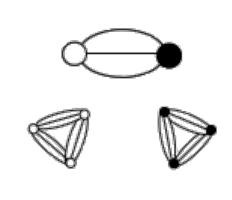
\includegraphics[width=\textwidth]{imgs/ep5-fig-7-7.pdf}
\captionof{figure}{Baryonenenstehung\\ aus Gluon-Jet \label{fig:7.7}}
\end{minipage}

\end{enumerate}
\end{itemize}
\newpage
\begin{itemize}
\item \tb{Farbe}
\begin{itemize}
\item[1.] \tb{Das $\Delta^{++}$-Baryon ($\Delta^{++}(1232))$}\\
Produktion z.B. $\nu_\mu p\rightarrow\mu^-\Delta^{++}$
\begin{align}
\ket{\Delta^{++}}=\ket{u\uparrow u\uparrow u\uparrow};\ J^p=(\frac{3}{2})^+
\end{align}
$\rightarrow$ Bahndrehimpuls $L=0$ (leichterer Q=2e-Baryon)\\
$\rightarrow$ Symmetrische Wellenfunktion (Flavour, Spin, Ort)
$\rightarrow$ symm. unter Tausch von 2 identischen Fermionen $\thor$ Pauli-Prinzip\\
$\rightarrow$ Lösung: $\ket{u_r\uparrow u_b\uparrow u_s\uparrow}$ mit antisymmetrischen Farb-Wellenfkt. %bin nicht sicher ob u_r stimmt konnte es nicht genau lesen!
\item[2.] \tb{WQ für $e^+ e^- \rightarrow q\bar{q} \rightarrow$ Hadronen} (z.B.: Abb.\ref{fig:7.8})
\begin{figure}[!ht]
\centering
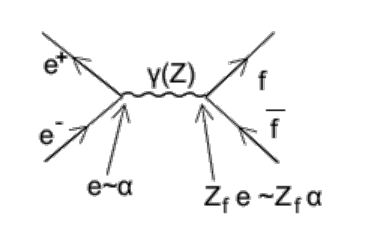
\includegraphics[width=.45\textwidth]{imgs/ep5-fig-7-8.pdf}
\caption{Feynmandiagramm zu $e^+e^-\rightarrow f\bar{f}$ \label{fig:7.8}}
\end{figure}

Diese Reaktion $e^+e^-\rightarrow \underbrace{f\bar{f}}_{\text{Fermion/Antifermion-Paar}}$ ist möglich wenn
\begin{align*}
s=(E_{cms})^2 > (2m_f)^2
\end{align*}
$Z^0$-Austausch dominant bei $\sqrt{s}=M_z$, aber klein bei $\sqrt{s}\approx \mathcal{O}(10\,keV)$\\
Wirkungsquerschnitt:
\begin{align}
\frac{\Pa \sigma}{\Pa \Omega}\sim \frac{Z^2_f\alpha^2}{s} (1+cos^2\theta)
\end{align}
Betrachte
\begin{align}
\Pa\frac{\sigma^{Had}}{\Pa\omega}=\sum_{\sqrt{s}>2m_{a_i}\footnotemark}\frac{\Pa \sigma^{a_i}}{\Pa \Omega}
\end{align}
Summenindex hat Schwelle bei $\sim$ 1\,GeV für strange-, $\sim$ 3\,GeV für charme-, $\sim$ 10\,GeV für bottom- und $\sim$ 350\,GeV für top-Quarks.\\
Verwende $e^+e^-\rightarrow\mu^+\mu^-$ als \grqq Eichreaktion\grqq:
\begin{align}
R_\mu=\frac{\nicefrac{d\sigma^{Had}}{d\Omega}}{\nicefrac{d\sigma^\mu}{d\Omega}}=\sum_{\sqrt{s}>2M_{a_i}}Z^2_{a_i}
\end{align}
Summieren über alle Farbzustände (r,g,b)$\rightarrow$ Faktor 3\\
Erhalten also:
\begin{align}\label{eq:7.8}
R_\mu = 3 \bigg[\underbrace{\underbrace{\underbrace{\underbrace{\stackrel{u}{\left(\frac{2}{3}\right)^2}+\stackrel{d}{\left(\frac{1}{3}\right)^2}}_{\sqrt{s}\geq 150\,MeV}+\stackrel{s}{\left(\frac{1}{3}\right)^2}}_{\sqrt{s}\geq 1\,GeV}+\stackrel{c}{\left(\frac{2}{3}\right)^2}}_{\sqrt{s}\geq 3\,GeV}+\stackrel{b}{\left(\frac{1}{3}\right)^2}}_{\sqrt{s}\geq 10\,GeV}+\stackrel{t}{\left(\frac{2}{3}\right)^2}\bigg]
\end{align}
\begin{figure}[!ht]
\centering
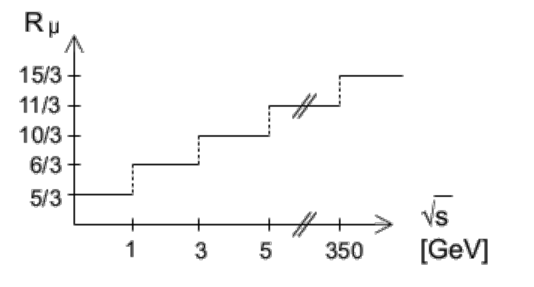
\includegraphics[width=.5\textwidth]{imgs/ep5-fig-7-9.pdf}
\caption{Graphische Veranschaulichung der Geichung \ref{eq:7.8} \label{fig:7.9}}
\end{figure}
\begin{itemize}
\item[$\rightarrow$] Faktor 3 durch Messung bestätigt
\item[$\rightarrow$] Es gibt Farbladungen und davor genannt
\end{itemize}
\end{itemize}
\end{itemize}
\section{Die starke Kopplung: Confinement und Asymptotic-Freedom}
Die Kopplungsstärke von Wechselwirkungen hängt von $Q^2$ ab. Grund sind höhere Ordnungen der Störungsreihe
\begin{itemize}
\item Für elektromagnetische WW (QED):
\begin{figure}[!ht]
\centering
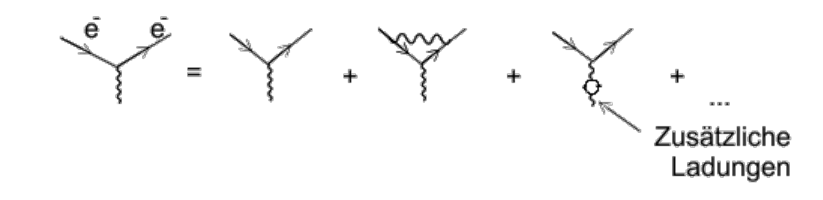
\includegraphics[width=.65\textwidth]{imgs/ep5-fig-7-10.pdf}
\caption{Höhere Ordnungen elektromagnetischer Wechselwirkung \label{fig:7.10}}
\end{figure}

$\Rightarrow$ Abschirmung:

\begin{figure}[!ht]
\centering
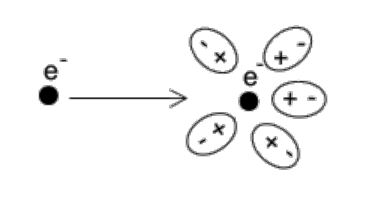
\includegraphics[width=.5\textwidth]{imgs/ep5-fig-7-11.pdf}
\caption{Dipolwolke um das rechte Elektron schirmt das linke, einfliegende Elektron ab \label{fig:7.11}}
\end{figure}

$\rightarrow$ Ladung umso größer, je \grqq näher man kommt \grqq\, d.h. desto größer $Q^2$
\begin{align}
\Rightarrow\alpha=\alpha(Q^2)=
\begin{cases}
\nicefrac{1}{137} & (Q^2=0)\\
\nicefrac{1}{128} & (Q^2=M^2_z)
\end{cases}
\end{align}

\item Für starke WW (QCD):

\begin{figure}[!ht]
\centering
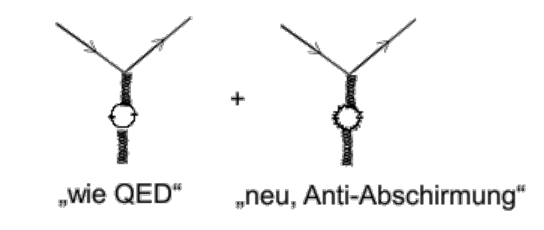
\includegraphics[width=.5\textwidth]{imgs/ep5-fig-7-12.pdf}
\caption{Höhere Ordnungen der starken Wechselwirkung \label{fig:7.12}}
\end{figure}
\begin{itemize}
\item[$\rightarrow$] dominant!
\item[$\Rightarrow$] $\alpha_s(Q^2)$ wird mit $Q^2$ kleiner!
\begin{align}
\Rightarrow \text{\fbox{$\alpha_s(Q^2)=\frac{12\pi}{(33-2N_f\footnotemark)ln\frac{Q^2}{\Lambda^2\footnotemark}}+h.O.$}} 
\end{align}
\begin{compactitem}
\item[mit] $N_f$: Zahl der Quarkflavours
\item[] $\Lambda$: in QED-Skala $\sim$ 250\,MeV
\end{compactitem}
\begin{align}
\alpha_s(Q^2)=
\begin{cases}
0,1185 & (Q^2=M^2_z)\\
0,3 & (Q^2=m^2_\tau)\\
>1 & (Q^2\leq 0,1\, GeV^2)
\end{cases}
\end{align}
\item[$\Rightarrow$] \textbf{Grenzfläche:}
\begin{itemize}
\item $Q^2\rightarrow 0:\ \alpha_s\rightarrow\infty$
\begin{itemize}
\item[$\rightarrow$] keine Störungsrechnung
\item[$\rightarrow$] keine freien Farbladungen
\item[$\rightarrow$] \grqq Confinement \grqq\
\end{itemize}
\item $Q^2\rightarrow \infty:\ \alpha_s \rightarrow 0$
\begin{itemize}
\item[$\rightarrow$] Störungsrechnung (QCD)
\item[$\rightarrow$] \grqq quasi-freie\grqq{} Quarks in tiefinelastischer Streuung
\item[$\rightarrow$] \grqq Asymptotic-Freedom\grqq\
\end{itemize}
\end{itemize}
\end{itemize}
\end{itemize}

\vorlesung{19. Januar 2018}

\section{Aufbau der Hadronen}
Quark-Gluon-Kopplung unabhängig von Quark-Flavour (u,d,s,c,t,b)
\begin{itemize}
\item[$\ra$] Hadron-Zustände nur von Bindungszustand ($L,J,n$) abhängig?
\item[$\ra$] Nein:            Effekt
\item[$\ra$] Quark-Massen     groß
\item[$\ra$] Quark-Ladungen   klein
\item \tb{Isospin-Symmetrie}\\
u- und d-Quarks haben etwa gleiche Massen (einige MeV)
\begin{itemize}
\item[$\Ra$]u$\leftrightarrow$d lässt die Hadronzustände \textbf{näherungsweise} invariant
\item[$\Ra$] Formel: starke WW \textbf{näherungsweise} invariant unter:
\begin{align*}
\left(\begin{array}{c}u\\d\end{array}\right)\rightarrow SU(2)\left(\begin{array}{c}u\\d\end{array}\right)\\
\Rightarrow \text{\grqq Isospin\grqq}\\
\ket{u}=I, I=\frac{1}{2}, \ket{_3=\frac{1}{2}}\\
\ket{d}=I, I=\frac{1}{2}, \ket{_3=-\frac{1}{2}}
\end{align*}
\item[$\Rightarrow$] Es gibt \grqq Sätze\grqq\ von Hadronen die aus $\stackrel{\leftrightarrow}{u},\stackrel{\leftrightarrow}{d}$ bestehen und mit $SU(2)$-Isospin in  sich selbst übergehen $\rightarrow$ \grqq Isospin-Multipletts\grqq
\begin{itemize}
\item gleiches $I$
\item $\sim$ gleiche Massen
\item Ladung = $f(I_3)$
\end{itemize}
\end{itemize}
$\Rightarrow$ Beispiel: Mesonen

\begin{figure}[!ht]
\centering
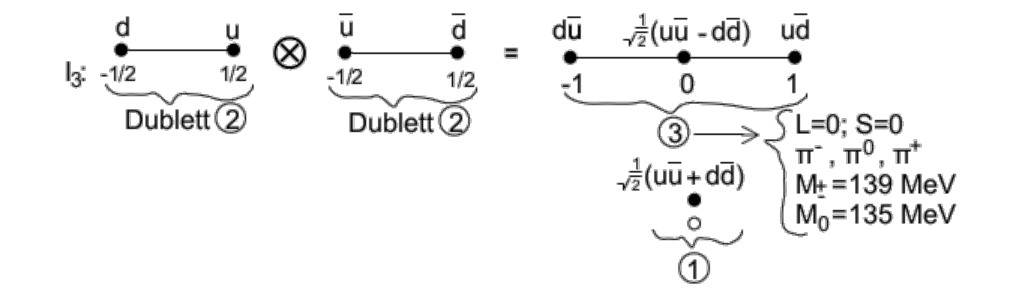
\includegraphics[width=.75\textwidth]{imgs/ep5-fig-7-13.pdf}
\caption{Isospinzusammensetzung bei Mesonen \label{fig:7.13}}
\end{figure}

Entstehendes Meson aus
\begin{align*}
L=0;\ S=0\rightarrow J^{PC}=0^{-+}:\ \pi^+,\pi^-,\pi^0\\
L=0;\ S=1\rightarrow J^{PC}=1^{--}:\ \rho^+,\rho^-,\rho^0\\
(M_\rho\approx 770\,MeV)
\end{align*}
\item \tb{Erweiterung auf 3 Quark-Flavours:}\\
$(u,d,s)$, $SU(2)\rightarrow SU(3),d.h.:$
\begin{figure}[!ht]
\centering
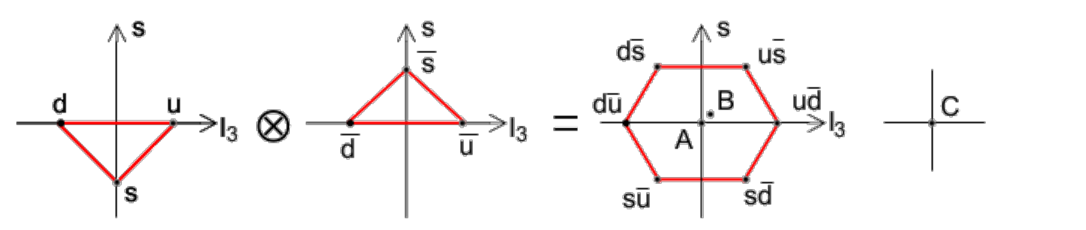
\includegraphics[width=.75\textwidth]{imgs/ep5-fig-7-14.pdf}
\caption{Erweiterung der Isopspinsymmetrie um den dritten Quarkflavour s \label{fig:7.14}}
\end{figure}
\begin{align}\begin{split}
A&=\frac{1}{\sqrt{2}}(u\bar{u}-d\bar{d})=\ket{\pi^0}\\
B&=\frac{1}{\sqrt{6}}(u\bar{u}+d\bar{d}-2s\bar{s})\approx\ket{\eta}\\
C&=\frac{1}{\sqrt{3}}(u\bar{u}+d\bar{d}+s\bar{s})\approx\ket{\eta^\prime}
\end{split}\end{align}
Wobei $B$ und $C$ mischen!

Wegen $m_s\gg m_{u,d}$: Massen \textbf{nicht} ähnlich $(M_\pi=139\,\mr{MeV},\ M_K=485\,\mr{MeV})$
\begin{itemize}
\item[$\Rightarrow$] SU(3) keine \grqq gute\grqq Symmetrie, aber bietet gute Ordnungsschema, auch für Baryonen
\end{itemize}
\item \tb{Erweiterung auf c-Quarks}
\begin{itemize}
\item[$\rightarrow$]$SU(3)\rightarrow SU(4)$
\item[$\rightarrow$] 3D-Multipletts
\item[$\rightarrow$] wichtig als Ordnungsschema
\end{itemize}
\end{itemize}

\section{Erzeugung und Zerfall von Hadronen}
\begin{itemize}
\item \tb{Erzeugung}\\
In hadronischen Reaktionen
\begin{itemize}
\item[$\ra$] \grqq Umwandlung von Quark-Linien\grqq\, z.B. $\pi^- p\rightarrow\pi^0 n$

\begin{figure}[!ht]
\centering
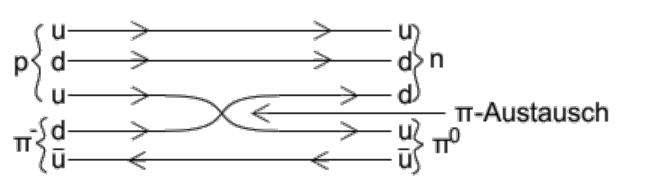
\includegraphics[width=.5\textwidth]{imgs/ep5-fig-7-15.pdf}
\caption{Feynmandiagramm zur Umwnadlungsreaktion \label{fig:7.15}}
\end{figure}

\item[$\ra$] Erzeugung/Vernichtung von Quark-Antiquark-Teilchen\\
z.B. $\pi^- p \rightarrow \Delta^0(1232)\rightarrow\pi^0 n$

\begin{figure}[!ht]
\centering
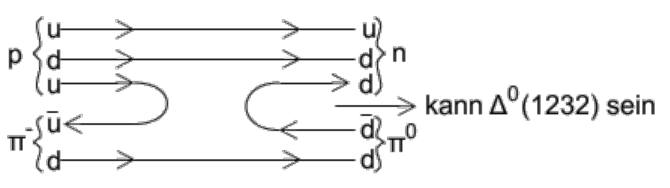
\includegraphics[width=.5\textwidth]{imgs/ep5-fig-7-16.pdf}
\caption{Feynmandiagramm zur $\pi^0n$ Erzeugung\label{fig:7.16}}
\end{figure}

z.B. $\pi^- p \rightarrow \Lambda k^0$
\begin{figure}[!ht]
\centering
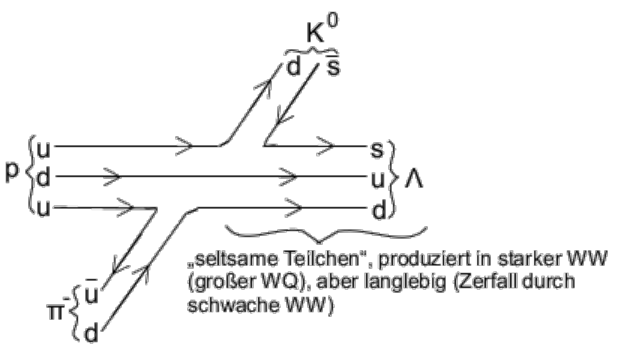
\includegraphics[width=.5\textwidth]{imgs/ep5-fig-7-17.pdf}
\caption{Assoziierte Produktion \label{fig:7.17}}
\end{figure}

\item[$\ra$] Inelastisch, z.B. in Jet-Bildung (\grqq Fragmentation\grqq, \grqq Hadronisation\grqq)
\end{itemize}
In $e^+ e^-$-Streuung:
\begin{itemize}
\item[$\ra$] Hadronische $q\bar{q}$-Resonanzen, z.B. $e^+ e^- \rightarrow \nicefrac{J}{\Psi}$

\begin{figure}[!ht]
\centering
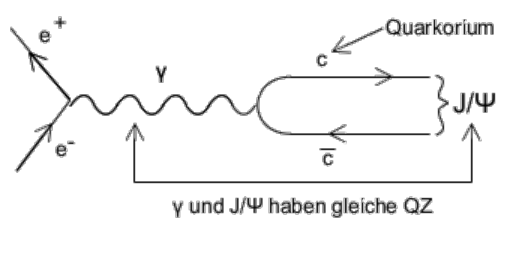
\includegraphics[width=.5\textwidth]{imgs/ep5-fig-7-18.pdf}
\caption{Inelastische Erzeugung von $\nicefrac J\Psi$ \label{fig:7.18}}
\end{figure}

Auch für
\begin{align*}
u\bar{u},d\bar{d}: \rho^0\\
s\bar{s}: \phi\\
b\bar{b}: \gamma 
\end{align*}
\item[$\ra$] $e^+ e^- \rightarrow qq(g)$, Jet-Bildung
\end{itemize}
%hier ist iwas zerschossenes es sieht auf jeden fall kackeeee aus
\item \tb{Zerfälle}\\
Alle 3 WW kommen vor
\begin{itemize}
\item[1.] starke WW, z.B. $\rho^0\rightarrow\pi^+\pi^-$
\begin{figure}[!ht]
\centering
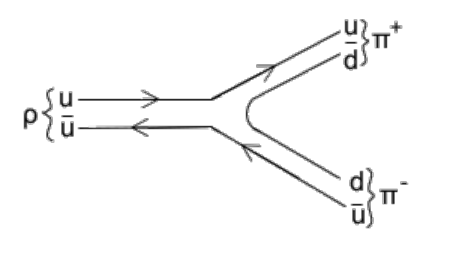
\includegraphics[width=.5\textwidth]{imgs/ep5-fig-7-19.pdf}
\caption{Zerfall von $\rho$ durch die starke WW \label{fig:7.19}}
\end{figure}

wenn erlaubt: dominant\\
Typisch : $\Gamma\approx 100...150\,\mr{MeV}$, $\tau\approx 10^{-23}\,\mr{s}$
\item[2.] Elektromagnetische WW (wenn Zerfall über starke WW nicht möglich ist)\\
z.B. $\pi^0\rightarrow\gamma\gamma$ (vgl. Abb. \ref{fig:7.20})

\begin{figure}[!ht]
\centering
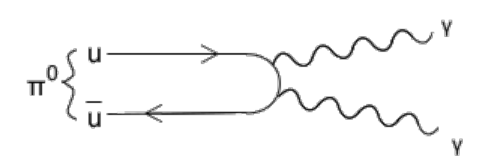
\includegraphics[width=.5\textwidth]{imgs/ep5-fig-7-20.pdf}
\caption{Zerfall von $\pi^0$ durch elektromagnetische WW \label{fig:7.20}}
\end{figure}

$\pi^0$ leichteres Hadron, starker Zerfall nicht möglich
$\tau\approx 10^{-16}\,\mr{s}$\\
auch: $\sum^0\rightarrow \Lambda\gamma$
\item[3.] schwache WW (wenn starke und elm. verboten sind)\\
Insbesondere für leichte/leichteste Hadronen mit $S\neq 0,C\neq 0, B\neq 0$\\
z.B. $K^+\rightarrow \mu^+\nu_\mu$ (vgl. Abb.\ref{fig:7.21})

\begin{figure}[!ht]
\centering
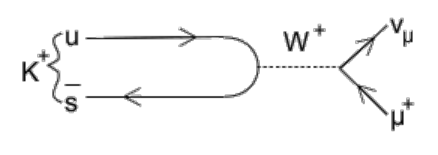
\includegraphics[width=.5\textwidth]{imgs/ep5-fig-7-21.pdf}
\caption{Zerfall von $K^+$ durch Austausch eines $W^+$-Bosons \label{fig:7.21}}
\end{figure}

genauso: $\Pi^+(s\leftrightarrow d)$
\item[$\rightarrow$] Spezieller Fall: Quarkonium\\
Zustände aus einem Quark und seinem Antiquark, Mesonen ohne elektrische Ladung oder Flavour.

Für die Lebensdauer gilt: $\tau \sim 0.7\cdot 10^{-20}\,s$ 

\begin{figure}[!ht]
\centering
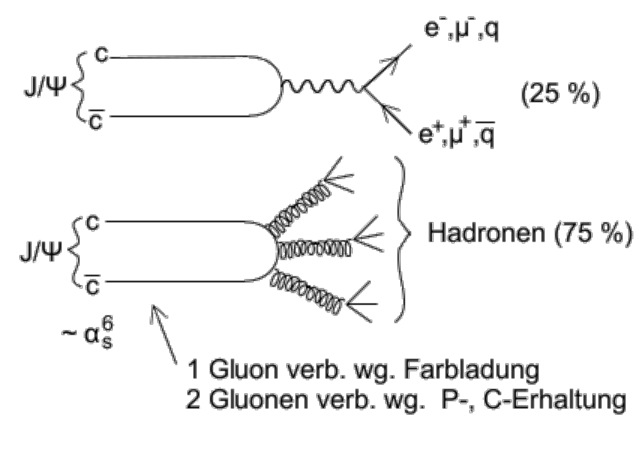
\includegraphics[width=.5\textwidth]{imgs/ep5-fig-7-22.pdf}
\caption{Feynmandiagramm zum Quarkonium \label{fig:7.22}}
\end{figure}
\end{itemize}
\end{itemize}
